\documentclass[9pt,a4paper,twocolumn,twoside]{rho-class/rho}

% --- 1. Idioma y matemáticas básicas ---
\usepackage[spanish,es-nodecimaldot,es-noindentfirst,es-noshorthands]{babel}

% --- 2. EL TRUCO DE MAGIA (BIEN ESCRITO) ---
% Borramos los comandos problemáticos usando su nombre exacto interno
\expandafter\let\csname not=\endcsname\relax
\expandafter\let\csname not<\endcsname\relax
\expandafter\let\csname not>\endcsname\relax

% Ahora ya podemos cargar la fuente moderna sin que explote
\usepackage{fontspec}
\usepackage{unicode-math}

% --- 3. Bibliografía ---
\addbibresource{rho.bib}

% --- 4. Datos del Informe ---
\title{Estudio de la radiación con el experimento de Geiger-Müller}
\author{Edgar Fernández Vigil}
\affil{Física - Facultad de Ciencias - Universidad de Oviedo}
\dates{\today}
\journalname{TEIII - Práctica de Laboratorio}
\journal{Radiación con el experimento de Geiger-Müller}

% --- 5. Resumen ---
\begin{abstract}
\noindent
En este informe se presenta el estudio experimental de la radiación ionizante utilizando un detector Geiger-Müller. En primer lugar, se caracterizó el dispositivo mediante la obtención de la curva \textit{plateau}, fijando un voltaje de operación de 1000 V para garantizar la estabilidad de las medidas. Se analizó la naturaleza estadística de las emisiones, comprobando que el fondo ambiental sigue una distribución de Poisson, mientras que las fuentes de alta actividad se aproximan a una distribución de Gauss. Además, se estudió la atenuación de la radiación con la distancia, verificando la necesidad de correcciones por ángulo sólido, y se midió el alcance de las partículas $\beta$ en aluminio. A partir del rango de frenado ($R \approx 849 \text{ mg/cm}^2$), se estimó una energía máxima de 1.856 MeV, lo que confirma la detección de electrones procedentes del isótopo hijo $^{90}\text{Y}$. Los resultados obtenidos presentan una alta coherencia con el \textbf{valor referencial} esperado, validando las leyes de interacción radiación-materia en el laboratorio.
\end{abstract}

% ----------------------------------------------------------
\begin{document}

    \maketitle
    \thispagestyle{firststyle}

\section{Introducción y motivación}

\rhostart{D}urante esta práctica trataremos de entender cómo funciona un detector Geiger-Müller para la medición de radiación ionizante en entornos de baja actividad. Para ello, analizaremos por partes cada uno de los fenómenos que afectan a la detección. 

En primer lugar, caracterizaremos el propio tubo, estudiando cómo se comporta la tasa de conteo al variar la diferencia de potencial para poder trabajar en un rango seguro y fiable. Además, estudiaremos el comportamiento estadístico de las emisiones. Como la desintegración es un proceso aleatorio, veremos en qué casos nuestras mediciones se ajustan a una distribución de Poisson (para el fondo ambiental) y en cuáles se acercan a una campana de Gauss (para fuentes muy activas). Por último, analizaremos cómo disminuye la cantidad de partículas detectadas al alejarnos de la muestra, y mediremos experimentalmente el poder de penetración de distintos tipos de radiación ($\alpha$, $\beta$ y $\gamma$) interponiendo distintos materiales absorbentes.

\section{Objetivos}

La finalidad general de esta práctica es familiarizarnos con los métodos de medida de radiación y comprender los efectos de la interacción radiación-materia. En concreto, buscaremos:

\begin{itemize}
    \item \textbf{Caracterizar el tubo Geiger-Müller:} Obtendremos la curva \textit{plateau} variando el voltaje para buscar el punto de operación óptimo y calcular la pendiente de la zona de trabajo.
    \item \textbf{Análisis estadístico:} Comprobaremos que la radiación de fondo sigue una estadística de Poisson y que las muestras de alta actividad se rigen por una distribución de Gauss.
    \item \textbf{Atenuación geométrica:} Demostraremos que la tasa de detección disminuye de forma proporcional a la inversa del cuadrado de la distancia ($\sim 1/d^2$).
    \item \textbf{Absorción de partículas $\beta$:} Calcularemos el coeficiente de absorción y el rango de frenado interponiendo láminas de aluminio, lo que nos permitirá estimar la energía máxima de la desintegración.
    \item \textbf{Radiación $\alpha$ y $\gamma$:} Analizaremos cualitativamente el poder de penetración de partículas alfa ($^{238}\text{Pu}$) y fotones gamma ($^{60}\text{Co}$).
\end{itemize}

\section{Dispositivo Experimental}

Para llevar a cabo las mediciones, montamos un dispositivo que consta del siguiente equipamiento:

\begin{itemize}
    \item \textbf{Tubo Geiger-Müller:} Detector cilíndrico de 1.43 cm de radio y 5.7 cm de longitud, conectado a un suministro de alta tensión (HV).
    \item \textbf{Contador digital:} Unidad SPECTEC conectada al PC que permite el control del voltaje y el registro de las cuentas.
    \item \textbf{Banco de muestras:} Soporte escalonado diseñado para colocar la fuente a distancias precisas, separadas por 1 cm.
    \item \textbf{Filtros:} Diferentes láminas de plomo y aluminio de espesor y densidad superficial conocidas.
    \item \textbf{Fuentes radiactivas:} Conjunto de emisores de distinta naturaleza: $^{90}\text{Sr}$ ($\beta$), $^{60}\text{Co}$ ($\gamma$), $^{238}\text{Pu}$ ($\alpha$) y $^{204}\text{Tl}$ ($\beta$).
\end{itemize}

\section{Procedimiento Experimental}

Procedimos a realizar la práctica dividiendo la toma de datos en varias etapas:

\subsection{Curva \textit{plateau}}
Para el apartado de la curva característica, procedimos a caracterizar el tubo midiendo en primer lugar la tasa de conteo al variar progresivamente la tensión. Partiendo de 700 V, incrementamos el potencial en pasos de 25 V hasta alcanzar los 1200 V, registrando las cuentas en intervalos de 30 segundos. Con estos datos identificamos la región de meseta y fijamos la tensión de trabajo para el resto de la práctica en 1000 V.

\subsection{Análisis estadístico}
A continuación, ajustamos el equipo para medir la radiación ambiental. Tomamos más de 100 mediciones rápidas de 2 segundos sin ninguna muestra radiactiva presente, con el fin de estudiar el ruido de fondo. Seguidamente, introdujimos la fuente activa de $^{90}\text{Sr}$ y realizamos más de 500 mediciones de 1 segundo para obtener datos suficientes y analizar la distribución de Gauss.

\subsection{Dependencia con la distancia}
Para estudiar la atenuación geométrica, utilizamos la fuente de $^{90}\text{Sr}$ y fuimos alejándola del detector bajando escalón a escalón en el soporte (en intervalos de 1 cm). En cada posición, tomamos 5 mediciones de 10 segundos para poder calcular un valor medio fiable y su incertidumbre.

\subsection{Absorción en la materia}
Por último, para analizar la absorción material, mantuvimos la fuente fija y fuimos añadiendo láminas de aluminio entre la muestra y el detector. Tomamos varias medidas para cada grosor de placa, repitiendo el proceso posteriormente con láminas de plomo.

\section{Resultados y Discusión}

\subsection{Determinación de la curva \textit{plateau}}

Procedimos a caracterizar el comportamiento del detector graficando las curvas de calibración para los diferentes radioisótopos. En las Figuras \ref{fig:plateau_sr_pu} y \ref{fig:plateau_tl_co} observamos la tasa de conteo en función del voltaje.

\begin{figure}[htbp]
    \centering
    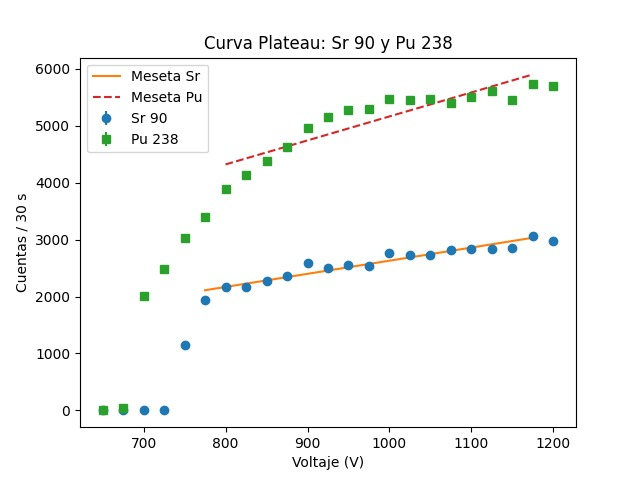
\includegraphics[width=\linewidth]{img/plateau-sr-pu.jpeg}
    \caption{Curvas \textit{plateau} para $^{90}\text{Sr}$ y $^{238}\text{Pu}$}
    \label{fig:plateau_sr_pu}
\end{figure}

Como podemos observar en la Figura \ref{fig:plateau_sr_pu}, las muestras de $^{90}\text{Sr}$ y $^{238}\text{Pu}$ presentan una alta actividad. Una vez superado el voltaje umbral, la tasa de cuentas se estabiliza. Al realizar el ajuste lineal en esta región de meseta, obtuvimos una pendiente de $2.31 \pm 0.17 \text{ cuentas/V}$ para el Estroncio y de $4.22 \pm 0.55 \text{ cuentas/V}$ para el Plutonio. Ambos valores cumplen el criterio teórico de presentar una variación inferior al 10\% por cada 100 V.

\begin{figure}[htbp]
    \centering
    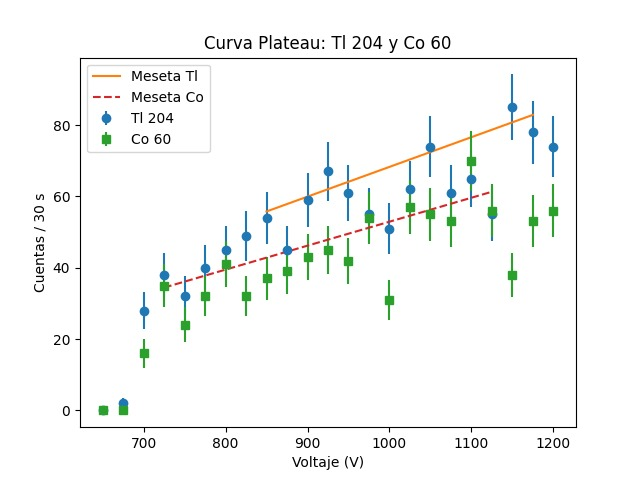
\includegraphics[width=\linewidth]{img/plateau-tl-co.jpeg}
    \caption{Curvas \textit{plateau} para $^{204}\text{Tl}$ y $^{60}\text{Co}$}
    \label{fig:plateau_tl_co}
\end{figure}

Por el contrario, al observar la Figura \ref{fig:plateau_tl_co}, vemos que la tasa de conteo es drásticamente inferior. Las pendientes obtenidas son casi nulas: $0.07 \pm 0.01 \text{ cuentas/V}$ para el Cobalto y $0.08 \pm 0.01 \text{ cuentas/V}$ para el Talio. Esta gran diferencia de cuentas en el $^{60}\text{Co}$ se debe a que la radiación $\gamma$ (fotones) tiene una probabilidad de interacción muy baja con el gas que rellena el tubo. En el caso del Talio, la baja actividad nos indica que la muestra se encuentra en un estado de decaimiento muy avanzado. En vista de los resultados, trabajar a 1000 V nos asegura estar operando dentro de la región de meseta para todas las muestras.

\subsection{Naturaleza estadística de la radiación}

Para entender mejor cómo fluctúa la medición de radiactividad, analizamos la dispersión de los datos recogidos en intervalos fijos de tiempo.

\begin{figure}[htbp]
    \centering
    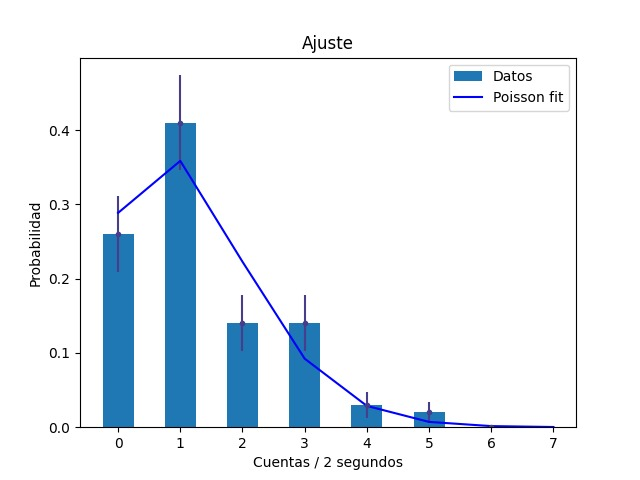
\includegraphics[width=\linewidth]{img/ajuste-poison.jpeg}
    \caption{Ajuste de la radiación de fondo (Poisson)}
    \label{fig:poisson}
\end{figure}

Al medir la radiación de fondo (Figura \ref{fig:poisson}), comprobamos que el histograma se ajusta perfectamente a una distribución de Poisson, arrojando un valor medio de $\mu = 1.24 \pm 0.02 \text{ cuentas/2s}$ y una desviación estándar de $\sigma = 1.11 \pm 0.13 \text{ cuentas/2s}$. Como la varianza ($\sigma^2 \approx 1.23$) es prácticamente igual a la media, confirmamos el carácter poissoniano del fondo. Conociendo las dimensiones del tubo, calculamos un área efectiva de $\approx 57.65 \text{ cm}^2$. Esto nos da como resultado un flujo de fondo de $0.64 \text{ incidentes/(cm}^2\cdot\text{min)}$, un valor que cuadra con la incidencia esperada de rayos cósmicos a nivel del mar.

\begin{figure}[htbp]
    \centering
    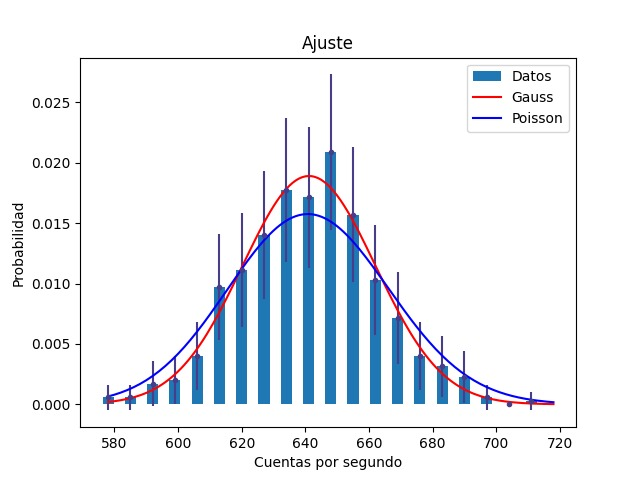
\includegraphics[width=\linewidth]{img/ajuste.jpeg}
    \caption{Comparativa de ajustes para una muestra activa}
    \label{fig:gauss}
\end{figure}

Sin embargo, cuando introducimos la fuente de $^{90}\text{Sr}$ en el detector (Figura \ref{fig:gauss}), el régimen cambia. Al procesar las cuentas, obtenemos una media muy elevada ($\mu = 641.2 \pm 0.8 \text{ cuentas/s}$). Debido a este gran número de eventos, la asimetría de Poisson desaparece y la distribución de los datos se ajusta con gran precisión a una campana de Gauss continua y simétrica, de acuerdo con el Teorema del Límite Central.

\subsection{Atenuación geométrica con la distancia}

A continuación, evaluamos la caída del flujo de partículas al separar progresivamente la fuente del detector.

\begin{figure}[htbp]
    \centering
    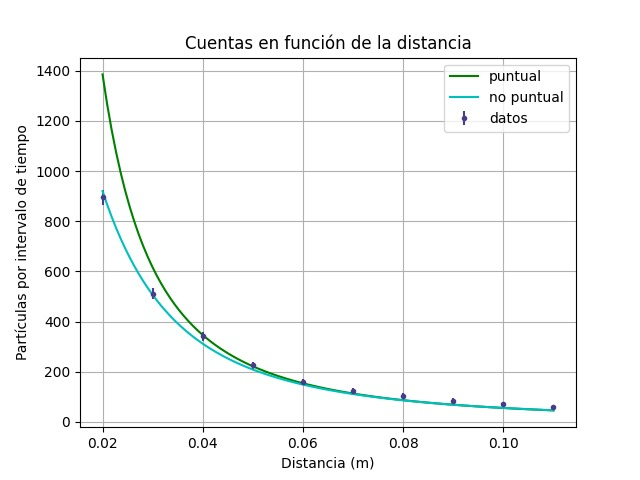
\includegraphics[width=\linewidth]{img/cuentas-distancia.jpeg}
    \caption{Tasa de conteo en función de la distancia}
    \label{fig:distancia}
\end{figure}

En la Figura \ref{fig:distancia} podemos observar que, al intentar ajustar los datos asumiendo que la fuente es un punto ideal (caída $1/d^2$), el ajuste se desvía considerablemente a distancias cortas. Para corregir esto, aplicamos un modelo "no puntual" que tiene en cuenta el ángulo sólido real de la ventana del Geiger. Este segundo ajuste funciona perfectamente y nos da un parámetro de actividad de $A = 7436.8 \pm 120.3 \text{ Bq}$. Sabiendo que la actividad teórica inicial de fábrica era de $3700 \text{ Bq}$ y que el isótopo se encuentra en equilibrio secular con el $^{90}\text{Y}$, el valor obtenido por nuestro ajuste resulta coherente con la actividad esperada.

\subsection{Absorción de partículas \texorpdfstring{$\beta$}{beta}}

Para el apartado de la atenuación material, implementamos el circuito de placas de aluminio con el objetivo de ver cómo el material iba frenando los electrones emitidos por el Estroncio.

\begin{figure}[htbp]
    \centering
    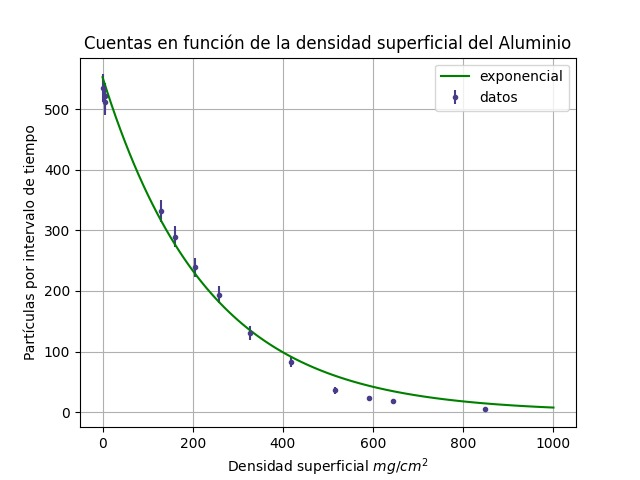
\includegraphics[width=\linewidth]{img/cuentas-densidad-superficial.jpeg}
    \caption{Cuentas detectadas en función del grosor de aluminio}
    \label{fig:absorcion_al}
\end{figure}

Tal y como se aprecia en la Figura \ref{fig:absorcion_al}, la tasa de cuentas decae de forma exponencial a medida que aumentamos la densidad superficial del absorbente. A partir del ajuste, calculamos un coeficiente de absorción másico de $\mu_m = 4.31 \text{ cm}^2/\text{g}$. 
Fijándonos en el punto donde la señal de las partículas se confunde con el ruido de fondo, estimamos un rango de frenado $R \approx 849 \text{ mg/cm}^2$. Utilizando la relación empírica para el aluminio ($E_{max} = 1.84 \cdot R + 0.294$), obtenemos una energía máxima de $1.856 \text{ MeV}$. Este resultado es muy revelador, ya que la energía de emisión del $^{90}\text{Sr}$ es de tan solo $0.546 \text{ MeV}$. Esto demuestra que estamos detectando principalmente las partículas de alta energía procedentes del decaimiento de su isótopo hijo, el $^{90}\text{Y}$ ($2.28 \text{ MeV}$).

\subsection{Apantallamiento de radiación \texorpdfstring{$\alpha$ y $\gamma$}{alfa y gamma}}

Por último, evaluamos el poder de penetración de otros tipos de radiación disponibles en el laboratorio. Al colocar la fuente de $^{238}\text{Pu}$ (que emite partículas alfa), observamos que bastaba con interponer una simple hoja de papel para que la tasa de detección cayera al nivel del fondo ambiental. Esto confirma el alcance extremadamente corto de este tipo de radiación masiva. 
Por el contrario, al medir el $^{60}\text{Co}$, comprobamos que los fotones gamma atravesaban el aluminio sin apenas sufrir atenuación, requiriendo láminas muy gruesas de plomo para notar una disminución significativa en las cuentas.

\section{Conclusiones}

En esta práctica se ha caracterizado el funcionamiento de un detector Geiger-Müller, determinando que su tensión de operación óptima se encuentra en torno a los 1000 V. Los resultados obtenidos para las curvas \textit{plateau} confirman que, en esta región de meseta, el detector es estable y presenta una pendiente de conteo inferior al 10\% por cada 100 V, lo cual es coherente con el \textbf{valor referencial} esperado para este tipo de instrumentación comercial.

El análisis estadístico ha permitido validar la naturaleza estocástica de la radiación. Se ha comprobado que el fondo ambiental sigue estrictamente una distribución de Poisson, mientras que las fuentes de mayor actividad, como el $^{90}\text{Sr}$, transicionan hacia una distribución gaussiana debido al elevado número de eventos registrados ($\mu \approx 641$ cuentas/s). Además, el estudio de la atenuación geométrica demostró que la aproximación de fuente puntual ($1/d^2$) falla a distancias cortas, siendo necesario aplicar una corrección por ángulo sólido para obtener un ajuste físicamente válido.

Finalmente, las pruebas de absorción han revelado las diferencias en el poder de penetración de las partículas $\alpha$, $\beta$ y $\gamma$. Un resultado especialmente relevante fue el cálculo del rango de frenado en aluminio ($R \approx 849 \text{ mg/cm}^2$), cuya energía máxima asociada ($1.856 \text{ MeV}$) confirma que en la muestra de Estroncio no solo detectamos el propio isótopo, sino principalmente las emisiones de alta energía de su hijo, el $^{90}\text{Y}$. En definitiva, la práctica ha servido para contrastar con éxito los modelos teóricos de interacción radiación-materia con las limitaciones y comportamientos reales observados en el laboratorio.

\appendix

\section{Cálculo de Incertidumbres}

Todo el tratamiento de datos y los ajustes de las gráficas presentadas en este informe se han programado mediante Python. Para calcular las incertidumbres hemos aplicado los siguientes criterios:

\subsection*{1. Incertidumbre estadística (Poisson)}
Dado que la desintegración radiactiva es un proceso aleatorio, asumimos que el número de cuentas registradas sigue una estadística de Poisson. Por lo tanto, para una única medición que registra $N$ cuentas (como hicimos en la curva \textit{plateau}), la incertidumbre asignada es directamente la raíz cuadrada del valor obtenido:
\vspace{0.2cm}
\begin{equation*}
    \delta N = \sqrt{N}
\end{equation*}

\subsection*{2. Incertidumbre en mediciones repetidas}
En los apartados de distancia y absorción, tomamos 5 medidas sucesivas ($N_1, \dots, N_5$) para cada punto y representamos la media $\bar{N}$.
Para asegurar una cota de error rigurosa, definimos la incertidumbre final como el valor máximo entre la predicción teórica de Poisson y la desviación estándar real de nuestras 5 mediciones:
\vspace{0.2cm}
\begin{equation*}
    \delta \bar{N} = \max \left( \sqrt{\bar{N}} \; , \; \sqrt{\frac{1}{n-1}\sum_{i=1}^{n} (N_i - \bar{N})^2} \right)
\end{equation*}
\vspace{0.2cm}

De esta forma, si el equipo o la medición tuvieron variaciones experimentales mayores a lo estadísticamente esperado, el error de nuestras gráficas las tendrá en cuenta.

\subsection*{3. Incertidumbre en histogramas}
Al representar las probabilidades ($p_i$) en los diagramas de barras de las distribuciones, donde se registran $c_i$ eventos sobre un total $N_{tot}$ de mediciones, el error asignado a cada barra se calculó como:
\vspace{0.2cm}
\begin{equation*}
    \delta p_i = \frac{\sqrt{c_i}}{N_{tot}}
\end{equation*}

\subsection*{4. Error de los parámetros de ajuste}
Para obtener variables como las pendientes, el parámetro geométrico $A$ o el coeficiente de absorción $\mu_m$, utilizamos las funciones de ajuste no lineal. El error reportado en el texto para cada variable se ha extraído directamente calculando la raíz cuadrada de la diagonal de la matriz de covarianza
\vspace{0.2cm}
\begin{equation*}
    \delta a_j = \sqrt{\Sigma_{jj}}
\end{equation*}

\end{document}